\documentclass{article}
\usepackage[utf8]{inputenc}
\parskip = 0.75em
\parindent = 10mm
\def\baselinestretch{1}
\usepackage {float}
\usepackage{listings}
\usepackage{subcaption}
\usepackage[usenames]{color}
\usepackage[numbers,sort&compress]{natbib}
\usepackage{multirow, array}
\usepackage[spanish]{babel}
	\deactivatetilden
	\spanishdecimal{.}
	\addto\captionsspanish{\def\tablename{Tabla}}
	\addto\captionsspanish{\def\listtablename{\'Indice de tablas}}

\usepackage{amsmath,amsfonts,amssymb}
	\allowdisplaybreaks[4]
\usepackage{graphicx}
	\graphicspath{{Figuras/}}
\usepackage[clearempty,pagestyles]{titlesec}
\usepackage{anysize}

\def\baselinestretch{1.5}
\papersize{27.9cm}{21.5cm} 
\marginsize{2cm}{2cm}{1cm}{1cm}

\begin{document}


	\begin{center}
	\huge{\textbf{Tarea 10 Algoritmo genético}}\\
	
	\textsc{ \Large Susana Ruiz Nuñez}
	\end{center}


\section{Planteamiento del problema} 
En esta práctica \cite{satu} se utiliza el problema de la mochila para implementar un algoritmo genético. Los algoritmos genéticos se suelen utilizar en casos donde no existe ningún algoritmo exacto eficiente, en esta práctica conviene comparar qué tan cerca a la solución óptima que da el algoritmo pseudo-polinomial, se logra llegar con un algoritmo genético. Un algoritmo genético representa posibles soluciones a un problema en términos de un genoma que en este caso va a ser un vector de verdades y falsos, indicando cuáles objetos se van a incluir en la mochila. Para esta práctica se pide cambiar la selección de padres para reproducción y que utilize selección de ruleta, cada solución se selecciona como padre con una probabilidad que es linealmente proporcional a su valor de función objetivo y a su factibilidad, combinando los dos a alguna función que parezca conveniente.

\section{Metodología}
Para desarrollar esta práctica primero se agrega al modelo ya existente \cite{satu} la selección de ruletas de la forma mencionada con anterioridad. Además se necesitó generar intancias con tres distintas reglas; Regla 1: el peso y el valor de cada objeto se generan independientemente con una distribución exponencial,
Regla 2: el peso de cada objeto se generan independientemente con una distribución exponencial y su valor es (positivamente) correlacionado con el peso, con un ruido normalmente distribuido de baja magnitud y
Regla 3: el peso de cada objeto se generan independientemente con una distribución exponencial y su valor es inversamente correlacionado con el peso, con un ruido normalmente distribuido de baja magnitud. 


\section{Resultados}

Se realizó el experimento que pedía incluir tres reglas nuevas de como eran generados los datos del peso y valor. Estos arrojaron un comportamiento en los datos para analizar detenidamente. Se muestra de forma clara que ya que se fortaleció el algoritmo con nuevas reglas y que se obtienen valores vs tiempo más elevados para la selección con ruleta. Se observa además que los mejores resultados se muestran para las reglas uno y tres. 

\begin{figure}
\centering
	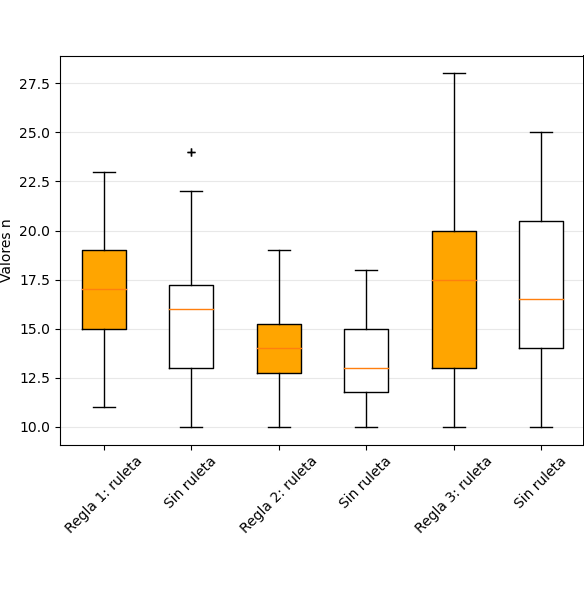
\includegraphics[scale=0.8]{Figure_1.png}
	\caption{Experimento con las tres reglas incluyendo selección de ruletas por valor obtenido por tiempo de ejecución.}
	\label{1}		
\end{figure}

\section{Pruebas Estadísticas}
Como se muestra en la Figura 2 a partir del décimoquinto paso para un total de cuarenta pasos realizados en el experimento no se observan cambios sustanciales en los dos métodos sin selección de ruletas y con selección de ruleta, incluso la selección sin ruleta muestra mejores resultados. 

\begin{figure}[H]
	\centering
	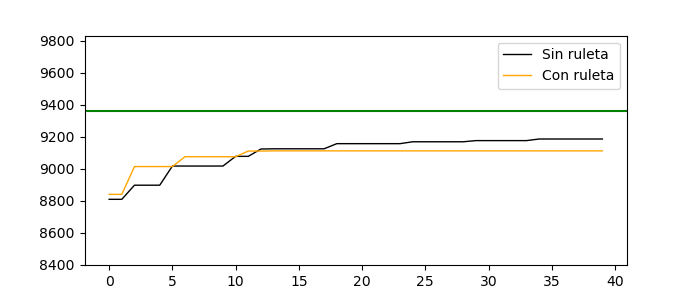
\includegraphics[scale=0.8]{Figure_2.png}
	\caption{Problema inicial con selección de ruleta incluido.}
	\label{1}		
\end{figure} 

Se realizaron pruebas estadísticas \cite{jason} para ver la relación existente entre los valores obtenidos en el experimento sin introducir la selección de ruleta y los valores cuando se introduce la selección de ruleta.

\subsection{Prueba de análisis de varianza (ANOVA)}
Se utiliza para comprobar si las medias de dos o más muestras independientes son significativamente diferentes. Prueba la relación  entre dos conjuntos de valores.

Supuestos
\begin{itemize}
	\item Las observaciones en cada muestra son independientes y están distribuidas de manera idéntica (iid).
	\item Las observaciones de cada muestra se distribuyen normalmente.
	\item Las observaciones en cada muestra tienen la misma varianza.
\end{itemize}

Interpretación
\begin{itemize}
	\item H0: las medias de las muestras son iguales.
	\item H1: una o más de las medias de las muestras son desiguales.
\end{itemize}

Resultados: Como el coeficiente de pearson p es mayor a 0.05 entonces se plantea que tienen probablemente la misma distribución.

\begin{lstlisting}[language=Python]
	stat=0.793, p=0.376
	Probably the same distribution
\end{lstlisting}


\section{Conclusiones}
Se concluye con los experimentos realizados que las reglas y el método de selección de ruleta agregaron robustez al algoritmo genético haciéndolo igual de competente que el método exacto. 

\bibliography{Tarea10}
\bibliographystyle{plainnat}
\end{document} 
